\documentclass[10pt, a4paper]{article}
% \usepackage[english]{babel}
\usepackage[brazilian]{babel}
\usepackage[utf8]{inputenc}
% \usepackage[T1]{fontenc}

% matlab code
% \usepackage{matlab-prettifier}
\usepackage[numbered,framed]{matlab-prettifier}
\renewcommand{\lstlistingname}{Anexo} % Listing->Code
\let\ph\mlplaceholder % shorter macro
\definecolor{codegreen}{rgb}{0,0.6,0}
\definecolor{codegray}{rgb}{0.5,0.5,0.5}
\definecolor{codepurple}{rgb}{0.58,0,0.82}
\definecolor{backcolour}{rgb}{0.95,0.95,0.92}
\lstdefinestyle{myStyle}{
    language=Matlab,
    breaklines=true,
    frame=single,
    numbers=none,
    basicstyle=\ttfamily\footnotesize,
%     basicstyle=\footnotesize\ttfamily,
    keywordstyle=\bfseries\color{magenta},
    commentstyle=\color{codegreen},
    identifierstyle=\color{blue},
    backgroundcolor=\color{backcolour},
    stringstyle=\color{codepurple},
}
\usepackage{adjustbox}

% For subfigure use
\usepackage[font=small,labelfont=bf]{caption}
\usepackage{subcaption}

% Set page size and margins
% Replace `letterpaper' with`a4paper' for UK/EU standard size
\usepackage[a4paper,top=2cm,bottom=2cm,left=2cm,right=2cm,marginparwidth=2cm]{geometry}

% tabelas
\usepackage{array}
\usepackage{tabularx}
\usepackage{booktabs}

\usepackage{float}

% Useful packages
\usepackage{amsmath}

\usepackage{graphicx}
%\graphicspath{{figures/}} %Setting the graphicspath
\usepackage[colorlinks=true, allcolors=blue]{hyperref}


\begin{document}

\begin{titlepage}
      \begin{center}
          \vspace*{1cm}

          \Huge
          \textbf{Lista 00}

          \vspace{0.5cm}
          \LARGE
          MEC 2403 - Otimização e Algoritmos para Engenhria Mecânica

          \vspace{1.5cm}

          \textbf{Pedro Henrique Cardoso Paulo \\ {\tt pedrorjpaulo.phcp@gmail.com}}

          \vfill
          Professor: Ivan Menezes

          \vspace{0.8cm}

          
\includegraphics[width=0.2\textwidth]{../general/puc.jpg}

          \Large
          Departamento de Engenharia Mecânica\\
          PUC-RJ Pontifícia Universidade Católica do Rio de Janeiro\\
          março, 2023

      \end{center}
  \end{titlepage}

% \maketitle

\section[q01]{Questão 01}

Para a questão 1 é solicitado calcular o gradiente e a metriz hessiana da função $f(x)$, dada por:

\begin{equation}
    f(x_1, x_2, x_3) = 3x_1^3x_2^2x_3 - 6x_1\log{x_2}x_3^4 + x_1^{-1}x_2^3 - x_1^2\sqrt{x_2}
\end{equation}

As derivadas de primeira ordem dessa função são dadas por:

\begin{equation}
    \frac{\partial f}{\partial x_1} = 9x_1^2x_2^2x_3 - 6x_3^4\log{x_2} - x_1^{-2}x_2^3 - 2x_1\sqrt{x_2}
\end{equation}

\begin{equation}
    \frac{\partial f}{\partial x_2} = 6x_1^3x_2x_3 - 6x_1x_2^{-1}x_3^4 + 3x_1^{-1}x_2^2 - \frac{x_1^2}{2\sqrt{x_2}}
\end{equation}

\begin{equation}
    \frac{\partial f}{\partial x_3} = 3x_1^3x_2^2 - 24x_1x_3^3\log{x_2}
\end{equation}

Já as derivadas segundas são dadas por:

\begin{equation}
    \frac{\partial^2 f}{\partial x_1^2} = 18x_1x_2^2x_3 + 2x_1^{-3}x_2^3 - 2\sqrt{x_2}
\end{equation}

\begin{equation}
    \frac{\partial^2 f}{\partial x_2^2} = 6x_1^3x_3 + 6x_1x_2^{-2}x_3^4 + 6x_1^{-1}x_2 + \frac{x_1^2}{4x_2\sqrt{x_2}}
\end{equation}

\begin{equation}
    \frac{\partial^2 f}{\partial x_3^2} = - 72x_1x_3^2\log{x_2}
\end{equation}

\begin{equation}
    \frac{\partial^2 f}{\partial x_1x_2} = 18x_1^2x_2x_3 - 6x_2^{-1}x_3^4 - 3x_1^{-2}x_2^2 - \frac{x_1}{\sqrt{x_2}}
\end{equation}

\begin{equation}
    \frac{\partial^2 f}{\partial x_1x_3} = 9x_1^2x_2^2 - 24x_3^3\log{x_2}
\end{equation}

\begin{equation}
    \frac{\partial^2 f}{\partial x_2x_3} = 6x_1^3x_2 - 24x_1x_2^{-1}x_3^3
\end{equation}

A partir dessas derivadas, definimos o gradiente ($\nabla f$) e a Hessiana ($\mathbf{H}$) como:

\[
  \nabla f =
  \left[ {\begin{array}{c}
    \frac{\partial f}{\partial x_1} \\
    \frac{\partial f}{\partial x_2} \\
    \frac{\partial f}{\partial x_3} \\
  \end{array} } \right]
  \]

\[
  \mathbf{H} =
  \left[ {\begin{array}{ccc}
    \frac{\partial^2 f}{\partial x_1^2} & \frac{\partial^2 f}{\partial x_1x_2} & \frac{\partial^2 f}{\partial x_1x_3} \\
    \frac{\partial^2 f}{\partial x_1x_2} & \frac{\partial^2 f}{\partial x_2^2} & \frac{\partial^2 f}{\partial x_2x_3} \\
    \frac{\partial^2 f}{\partial x_1x_3} & \frac{\partial^2 f}{\partial x_2x_3} & \frac{\partial^2 f}{\partial x_1^2} \\
  \end{array} } \right]
\]

\section[q02]{Questão 02}

O enunciado solicita classificar a metriz abaixo segundo sua positividade:

\[
  \mathbf{A} =
  \left[ {\begin{array}{ccc}
    3 & -2 & 1 \\
    -2 & 4 & -3 \\
    1 & -3 & 2 \\
  \end{array} } \right]
\]

A determinação da positividade da matriz será feita por meio de seus autodeterminantes. 
Caso os 3 autodeterminantes da matriz sejam positivos, sabe-se que ela será positiva definida. 
Caso eles alternem entre valores positivos e negativos, sabe-se que ela será negativa definida. Caso contrário,
nada pode-se afirmar. Calculando o primeiro:

\[
  \left| {\begin{array}{c}
    3\\
  \end{array} } \right| = 3
\]

Calculando o segundo:

\[
  \left| {\begin{array}{cc}
    3 & -2 \\
    -2 & 4 \\
  \end{array} } \right| = 8
\]

Calculando o terceiro:

\[
  \left| {\begin{array}{ccc}
    3 & -2 & 1 \\
    -2 & 4 & -3 \\
    1 & -3 & 2 \\
  \end{array} } \right| = -3
\]

Como nenhum dos padrões descritos foi respeitado, a matriz não é nem positiva definida e nem negativa definida, 
ou seja, a matriz apresenta autovalores positivos e negativos.

\section[q03]{Questão 03}

\begin{figure}
    \centering
    \begin{subfigure}[b]{0.45\textwidth}
        \centering
        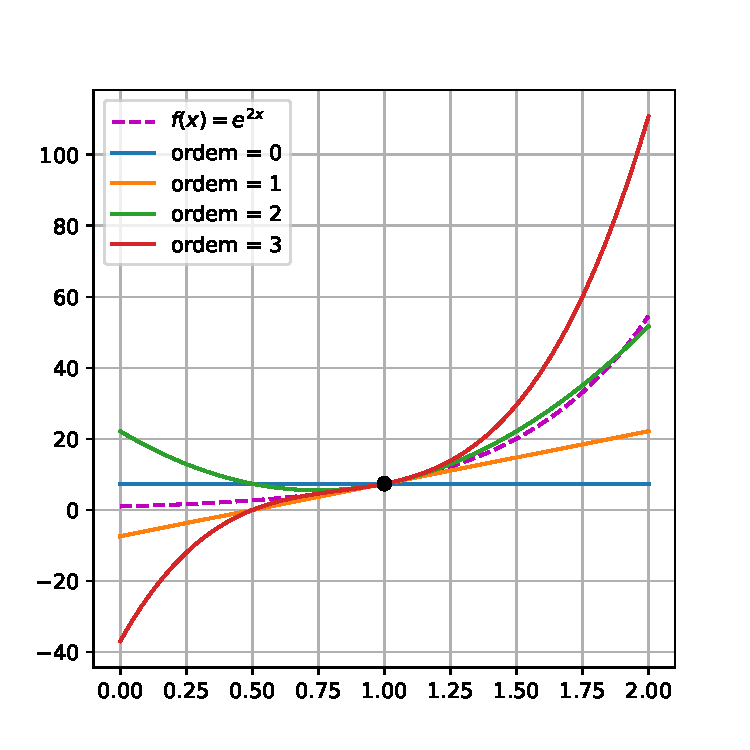
\includegraphics[width=\textwidth]{images/q3_1.pdf}
        \caption{$x \in [0, 2]$}
        \label{fig:q3_1}
    \end{subfigure}
    \hfill
    \begin{subfigure}[b]{0.45\textwidth}
        \centering
        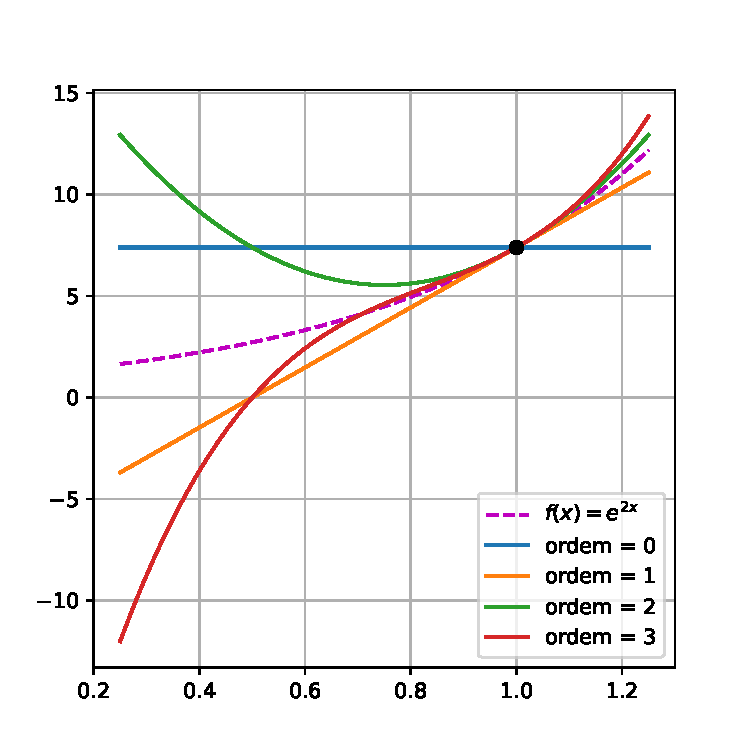
\includegraphics[width=\textwidth]{images/q3_2.pdf}
        \caption{$x \in [0.25, 1.25]$}
        \label{fig:q3_2}
    \end{subfigure}
    \hfill
    \begin{subfigure}[b]{0.45\textwidth}
        \centering
        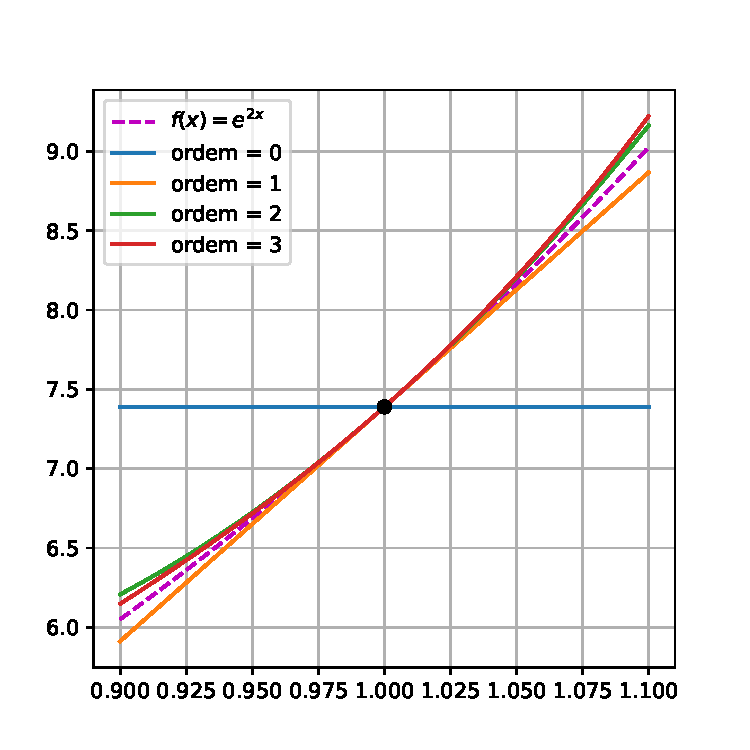
\includegraphics[width=\textwidth]{images/q3_3.pdf}
        \caption{$x \in [0.9, 1.1]$}
        \label{fig:q3_3}
    \end{subfigure}
       \caption{Função $f(x) = e^{2x}$ e seus polinômios de Taylor}
       \label{fig:q3}
\end{figure}

\section[q04]{Questão 04}

\bibliographystyle{apalike}
\bibliography{export}

\end{document}